\setlength\intextsep{1mm}

\section*{\textbf{Task 1: Implement PCA}}

% Implement the PCA algorithm using the given 2-d data (download the data here). Reproduce the illustrations shown in the figure below. You may use the implementation given in the slides as a basis for your work. 
% In the 1st figure, show the mean-centered data along with its two principal components (pointing in the two orthogonal directions of greatest variance in the dataset).
% In the 2nd figure, show the encoded version of the data in a space where the principal components are in line with the coordinate axes.
% -	Briefly describe how you implement PCA. You may include equations in your report to help with your explanation.
% -	A figure that shows the mean-centered data along with its two principal components. In the figure, include the data points and arrows indicating the two principal components.
% -	A figure that shows the encoded version of the data in a space where the principal components are in line with the coordinate axes. In the figure, include the data points and arrows indicating the two principal components.
\textbf{1.} Explanation of my implementation procedure

My implementation of PCA consists of the following steps:
\begin{itemize}
    \item Center the original data points x (x has a dimension of N*P, N: dimensional of each point/vector, P: number of data sample): $\textbf{X} = x - \bar{x}$
    \item Calculate the covariance matrix of $\textbf{X}$: $ Cov(\textbf{X}) = \frac{1}{P} \textbf{X} \textbf{X}^T $
    \item Perform eigendecomposition of the covariance matrix: $ Cov(\textbf{X}) = \frac{1}{P} \textbf{X} \textbf{X}^T = \textbf{V} \textbf{D} \textbf{V}^T$. The \textbf{V} is the eigenvectors and \textbf{D} is the eigenvalues.
    \item Perform dot product of \textbf{V} and \textbf{X} to get encoded data points $ w_p $: $ w_p = \textbf{V}^T \cdot \textbf{X}$
\end{itemize}


\textbf{2.} A figure that shows the mean-centered data along with its two principal components. And A figure that shows the encoded version of the data in a space where the principal components are in line with the coordinate axes. Red arrows show the principle components.

\begin{figure}[H]
    \centering
    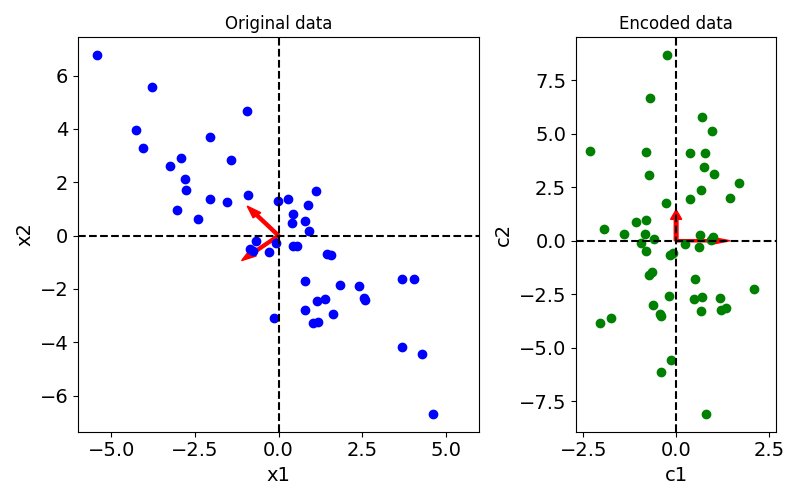
\includegraphics[width=120mm]{task1.png}
    \caption{PCA analysis}
    \label{fig:task1}
\end{figure}


\newpage
\section*{\textbf{Task 2: Implementing K-Means }}
% Implement the K-means algorithm and apply it to properly cluster the given dataset using K=3 cluster centroids. 

% 1.	Visualize your results by plotting the clustered dataset, coloring each cluster using a unique color. You might want to try to run the k-mean algorithm multiple times for each value of K to mitigate the bad initialization problem. 
% 2.	Make a scree plot by varying the number of clusters from 1 to 10. You might want to try to run the k-mean algorithm multiple times for each value of K to mitigate the bad initialization problem. Your scree plot should look like this: 

% -	Describe how you initialized the centroids and why you choose this method.
% -	A figure that visualizes your clustering results when K=3. To be more specific, you should color each cluster and put labels to indicate the clusters in the figure (not in the report). You should also highlight the centroid of each cluster and put labels to indicate the centroids as well.
% -	Scree plot by varying the number of clusters from 1 to 10. Based on the plot, answer what is the best K for this problem and why.


\textbf{1.} Describe the initialization process of the centroids and reasons.

Given each data point is a two dimensional vector, the centroids are generated randomly in the range of $[ x_{min}, x_{max} ] $ of each dimension. As we all know, the k-means method is sensitive to the initialization of centroids. In my procedure, I added 5 iterations (repeats) and each iteration will generate a new set of randomized starting centroids. The best initialization (with the lowest cost) will be picked as the final decision.


\textbf{2.} A figure that visualizes your clustering results when K=3.
\begin{figure}[H]
    \centering
    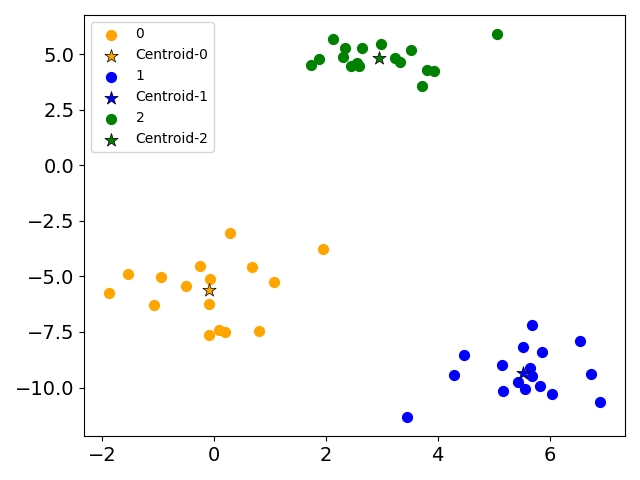
\includegraphics[width=100mm]{task2-cennum3.png}
    \caption{K-means clustering when centroid number = 3}
    \label{fig:task2-1}
\end{figure}

\textbf{2.} A figure showing the cost with varying number of clusters from 1 to 10.
\begin{figure}[H]
    \centering
    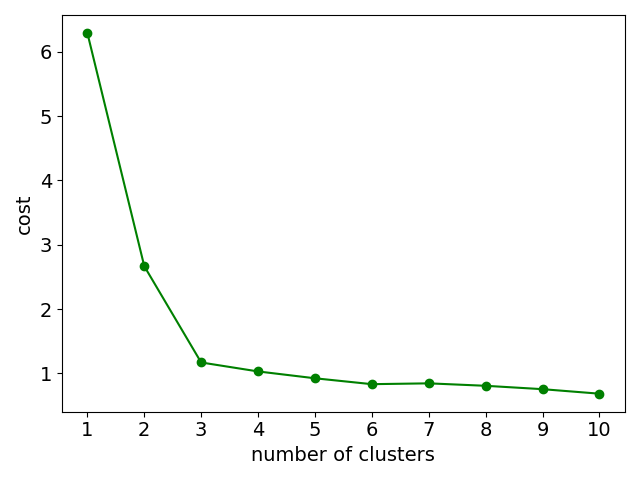
\includegraphics[width=100mm]{task2-cluster-numbers.png}
    \caption{K-means clustering when centroid number ranging from 1 to 10}
    \label{fig:task2-2}
\end{figure}

Based on Figure 3, I think K = 3 is the best option since the cost with K =3 lies in the "knee" point. With further adding more clusters, not much decreasing of the cost was gained.

